\documentclass[titlepage]{report}
\title{Amazon Web Services:\\ EC2\hyp{}virtual\hyp{}server und EC2\hyp{}container \\
\small Eine Seminar\hyp{}Arbeit bei Prof. Dr. -Ing. Dr. rer. nat. habil. \\
Harald Richter}
\usepackage[ngerman]{babel}
\usepackage[backend=biber,style=numeric]{biblatex}
\addbibresource{literature.bib}
\usepackage{caption}
\usepackage{subcaption}
\usepackage{graphicx}
\usepackage[utf8]{inputenc}
\usepackage[T1]{fontenc}
\usepackage{url}
\usepackage{hyphenat}
\author{Christian, Rebischke}
\begin{document}
\maketitle
\tableofcontents
\chapter*{Einleitung}
\addcontentsline{toc}{chapter}{Einleitung}
Im Zeitalter immer fortschreitender Digitalisierung wächst die Nachfrage
nach günstigem Speicherplatz und Rechenpower zunehmends. Der Trend geht
deshalb immer mehr zum Cloud Computing.  ``Zwei von drei Unternehmen (65
Prozent) haben in Deutschland im Jahr 2016 Cloud Computing
eingesetzt.''\footcite{SWG17} Cloud Computing ist die Möglichkeit
Speicher und Rechenpower in Form von Cloud\hyp{}Storage, virtuellen Servern,
der neuen Container\hyp{}Technologie oder ganzen Rechenzentren on\hyp{}demand
virtuell abzurufen, zu verwalten und für die eigene Firma möglichst
schlagkräftig zu verwenden. Die Vorteile dieses neuen Marktsegments sind
offensichtlich. So lassen sich Anwendungen jederzeit und an jedem Ort
der Welt deployen und einfach skalieren, so fern es der Cloud\hyp{}Anbieter
möglich macht durch Rechenzentren, verteilt über den gesamten Globus.
Dies ermöglicht ein rasantes Wachstum für neue Startups, kleine und
mittelständische Unternehmen sowie große Konglomerate wie Amazon oder
Microsoft wie es die Welt noch nie zuvor gesehen hat. Startups oder
bereits etablierte Firmen sparen sich auf diesem Wege den Overhead
eigene Hardware zu kaufen und zu verwalten.  Eigene Hardware hat den
Nachteil der Skalierbarkeit. Als Startup mit beispielsweise gerade mal
ein Dutzend Mitarbeitern ist es unmöglich weltweit zu skalieren auf
Basis von Hardware. Der Einkauf und die anschließende Verwaltung von
Servern, Routern, Storages oder Switches ist nicht nur kostenintensiv,
sondern vorallem auch zeit\hyp{} und Mitarbeiterintensiv.\footcite[S.
1]{RZ17} Besonders wenn man weltweit expandieren möchte ist es enorm
schwerig für Newcomer genug Infrastruktur aufzubauen um alle Kunden
zufriedenstellend zu versorgen.  So kann zum Beispiel eine Verbindung
zwischen dem Rechenzentrum einer Firma in München und einem Kunden in
Berlin zufriedenstellend sein. Ein Kunde in Asien jedoch, beispielsweise
China, hätte mit starker Latenz zu kämpfen. Ein weiteres Beispiel
Redundanz: Mit steigender Kundschaft steigt auch die Wahrscheinlichkeit
das Server ausfallen. Das kann viele Gründe haben. Hardware\hyp{}Ausfall,
Fehler in der Administration oder Überlastung wegen eines zu hohen Loads
auf dem Server sind nur wenige Gründe. Die Antwort darauf ist
horizontales Skalieren. Anstatt vertikal zu skalieren und mehr
Rechenpower und Speicher in nur eine Server\hyp{}Einheit zu stecken ist es
ratsamer die Last und damit auch das Ausfall\hyp{}Risiko auf mehrere Servern
zu verteilen. Im Idealfall sind diese Server sogar noch physisch von
einander getrennt um Ausfälle durch Naturkatastrophen oder politischen
Auseinandersetzungen zu vermeiden.  Alle diese Ansätze vereint Amazon
Web Services (AWS). Im weiteren Verlauf dieser Arbeit wird der Dienst
Amazon EC2 genauer vorgestellt und dessen Kernkonzepte Virtual\hyp{}Server
und Container genauer beleuchtet. Außerdem werden etwaige Vorteile und
Nachteile sowie Unterschiede zwischen beiden Konzepten hervorgehoben.
\begin{figure}[h]
    \centering
    \includegraphics[width=1.0\textwidth]{figures/scalability.pdf}
    \caption{Verdeutlichung Horizontaler Skalierung}\label{fig:1}
\end{figure}
\chapter*{Amazon EC2}
\addcontentsline{toc}{chapter}{Amazon EC2}
\section*{Einführung in Amazon EC2}
\addcontentsline{toc}{section}{Einführung in Amazon EC2}
Amazon EC2, ausgeschrieben Amazon Elastic Compute Cloud, ist im Jahr
2006 als Bestandteil von Amazon Web Services (AWS)
entstanden.\footcite{aws} Amazon Web Services gehört dem gleichnamigen
Tochterunternehmen des Online\hyp{}Versandhändlers Amazon.com.\footcite{Fou}
Das Tochterunternehmen deckt verschiedene Sparten des Cloud\hyp{}Computing
ab. Darunter fallen diverse Bereiche wie Rechenpower in Form von
virtuellen Servern und Containern, Speicher in Form des Amazon Web
Service S3 (Simple Storage Service) oder des Datenbank\hyp{}Services Amazon
RDS (Relational Database Service) oder Netzwerk in Form von CloudFront,
einem Content Delivery Network von Amazon Web Services. Weitere Dienste
sind zum Beispiel IAM (Identity and Access Managament), Lightsail oder Beanstalk.
Damit sind noch lange nicht alle Services genannt. In dieser Arbeit soll
es aber explizit um Amazon EC2 (Elastic Compute Cloud) gehen. Einige der
Hauptmerkmale von Amazon Elastic Compute Cloud sind:
\begin{itemize}
    \item Hohe Skalierbarkeit
    \item Webservice mit API
    \item Instanzen sind On\hyp{}Demand verfügbar innerhalb von Minuten anstatt
      Stunden oder Tagen
    \item Service Level Agreement garantiert 99,95\% uptime\footcite{ec2}
    \item Rechenzentren in verschiedenen Regionen der Welt
    \item Integration in andere Amazon Web Services: Zum Beispiel S3
    \item Kostengünstig: Es wird nur für genutzte Rechenkapazität bezahlt
\end{itemize}
Wenn man von Amazon EC2 spricht, spricht man fast immer von virtuellen
Maschinen in der Amazon Web Services Cloud. Als Grundlage für diese
virtuellen Maschinen oder auch Instanzen (englisch Instance) dienen
Amazon Machine Images (AMI).\footcite{ec2details} Amazon Machine
Images können verschiedene Betriebssysteme beinhalten. Angefangen bei
Microsoft Windows über diverse Linux Derivate wie Red Hat Linux (RHEL),
Debian oder CentOS. Anhand von diesen AMIs lassen sich dann wiederum
Instanzen starten. Kosten werden nur verursacht während eine Instanz
gestartet ist. (Bei einigen Amazon Machine Images können Lizenzkosten
anfallen, zum Beispiel Windows). Desweiteren lassen sich Amazon Machine
Images beliebig konfigurieren. Diese Konfiguration umfasst aber nur
Einstellungen auf Betriebssystemebene. Um Parameter wie CPU, RAM,
Speicher oder Netzwerk einzustellen bietet Amazon Web Services eine
Palette von Instanztypen (englisch Instance\hyp{}Types) an.
Diese Instanztypen decken ein breites Spektrum von unterschiedlichen
Konfigurationen ab. Angefangen beim kleinsten Instanztyp dem T2.nano mit
einem virtuellen CPU\hyp{}Kern und 0.5GiB Arbeitsspeicher bis hin zum größten
Instanztyp wie dem m4.16xlarge mit 64 virtuellen CPU\hyp{}Kernen, 256GiB
Arbeitsspeicher und einer dedizierten EBS\hyp{}Bandbreite von 10.000 Mbit/s.
\footcite{instance} EBS steht für Elastic Block Store und ist eine
dedizierte Speichereinheit in der Amazon Web Services Cloud. Elastic
Block Store kann auf jede beliebige Größe angepasst werden und ist
unabhängig von der Elastic Compute Cloud. So überlebt Elastic Block
Store beispielsweise einen Reboot der virtuellen Maschine und kann auch
an andere Instanzen angedockt/gemounted werden. Durch diese Eigenschaft
ist es möglich ohne Probleme innerhalb von Minuten von einer Instanz auf eine andere
umzuziehen.
\begin{table}[h]
    \centering
    \caption{Beispiel für die Varianz der Instanzen anhand vom Typ T2\footcite{Instance}}
    \label{tab:1}
\begin{tabular}{|c|c|c|c|c|}
\hline
Modell     & vCPU & CPU\hyp{}Guthaben/Stunde & Arbeitsspeicher (GiB) & Speicherung \\ \hline
t2.nano    & 1    & 3                   & 0.5                   & Nur EBS     \\
t2.micro   & 1    & 6                   & 1                     & Nur EBS     \\
t2.small   & 1    & 12                  & 2                     & Nur EBS     \\
t2.medium  & 2    & 24                  & 4                     & Nur EBS     \\
t2.large   & 2    & 36                  & 8                     & Nur EBS     \\
t2.xlarge  & 4    & 54                  & 16                    & Nur EBS     \\
t2.2xlarge & 8    & 81                  & 32                    & Nur EBS     \\ \hline
\end{tabular}
\end{table}
\begin{figure}[h]
    \centering
    \includegraphics[width=1.0\textwidth]{figures/EC2-Landscape.pdf}
    \caption{Übersicht über die EC2\hyp{}Instanz\hyp{}Landschaft}\label{fig:2}
\end{figure}
\section{Regionen}
Um eine weitgefächerte Verfügbarkeit und Skalierbarkeit zu gewährleisten
hat Amazon Web Services Rechenzentren in einem Dutzend Ländern. Dadurch
ist es möglich die Latenz und Fehlerquote von Webseiten und internetbasierten
Anwendungen so klein wie möglich zu halten. Dies hat nicht nur eine
höhere Kundenzufriedenheit zur Folge sondern hat auch technische
Vorteile (beispielsweise für Video\hyp{}Anwendungen). Zur Zeit unterhält
Amazon Web Services Rechenzentren in den folgenden Ländern:
\begin{itemize}
    \item USA
    \item Deutschland
    \item Volksrepublik China
    \item Irland
    \item Großbritannien
    \item Indien
    \item Südkorea
    \item Australien
    \item Japan
    \item Singapur
    \item Kanada
    \item Brasilien
\end{itemize}
Diese Länder sind eingeteilt in folgende geographische Regionen:
\begin{itemize}
    \item Nordamerika
    \item Europa/Naher Osten/Afrika
    \item Asien/Pazifik
    \item Südamerika
\end{itemize}
Damit sind bis auf den Kontinent Afrika, alle besiedelten Kontinente
abgedeckt. Diese geographischen Regionen sind dann nochmal in Regionen
unterteilt. Für Nordamerika wären das beispielsweise\footcite{region}:
\begin{itemize}
    \item USA Ost (Nord\hyp{}Virginia)
    \item USA Ost (Ohio)
    \item USA West (Oregon)
    \item USA West (Nordkalifornien)
    \item Kanada
    \item AWS GovCloud
\end{itemize}
AWS GovCloud ist eine Sonder\hyp{}Region und isoliert von allen anderen
Regionen. Der Grund dafür ist, dass AWS GovCloud Applikationen und
Informationen der US\hyp{}Regierung hosted.\footcite{govcloud} Zusätzlich zu
diesen Regionen gibt es noch sogenannte High\hyp{}Availability\hyp{}Zones
(Hoch\hyp{}Verfügbarkeits\hyp{}Zonen). Eine Region kann mehrere dieser
High\hyp{}Availability\hyp{}Zonen haben. Im Endeffekt handelt es sich bei
diesen Zonen um physische Rechenzentren in verschiedenen Städten innerhalb
einer Region. Die Region USA Ost (Nord Virginia) hat beispielsweise 5
High\hyp{}Availability\hyp{}Zonen. Durch diese
High\hyp{}Availability\hyp{}Zonen kann man Applikationen mehrfach in einer
Region deployen, dadurch erhält man automatische, unterbrechungsfreie Failover
die zu einer hohen Redundanz führen.\footcite{region} Realisiert wird dies
durch private Glasfasernetzwerke zwischen den einzelnen
High\hyp{}Availability\hyp{}Zonen. Dies lässt sich dann weiter hochskalieren
über ganze Regionen. Außerdem gibt es noch sogenannte
AWS\hyp{}Edge\hyp{}Network\hyp{}Standorte. Dies sind meistens Standorte für
Content\hyp{}Delivery-Netzwerke, kleinere Rechenzentren oder
Peering\hyp{}Endpunkte.
\section{Virtualisierung}
Einer der Schlüsselfaktoren für die gute Skalierbarkeit von Amazon EC2
ist die Virtualisierung. Durch den Einsatz von Virtualisierung ist es
möglich mehrere virtuelle Hosts auf einer Hardware laufen zu lassen.
Das Prinzip dahinter ist relativ simpel. Auf dem OS der Hardware läuft
ein Hypervisor oder auch Virtual Machine Monitor (VMM). Über diesen
Hypervisor können dann mehrere Instanzen von virtuellen Servern auf der
selben Hardware gestartet werden. Der Hypervisor gaukelt den einzelnen
Maschinen also vor, sie wären nur auf einem System.
\begin{figure}[h]
    \centering
    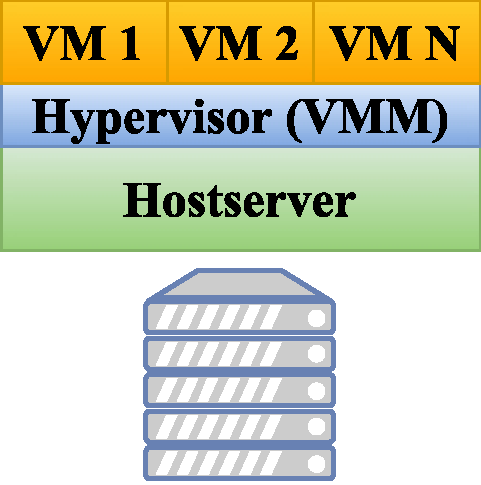
\includegraphics[width=0.5\textwidth]{figures/hypervisor.pdf}
    \caption{Visualisierung der Hypervisor-Technologie}\label{fig:3}
\end{figure}
Amazon Machine Images unterstützen zwei verschiedene Arten von
Virtualisierung:
\begin{itemize}
    \item paravirtual (PV)
    \item hardware virtual machine (HVM)
\end{itemize}
``Der Hauptunterschied zwischen PV und HVM basierten Amazon Machine
Images besteht im verwendeten Bootloader und der Verfügbarkeit von
speziellen Hardware-Erweiterungen (CPU, Netzwerk, Speicher) für bessere
Performance.''\footcite{virtualization} Bei PV basierten Amazon Machine
Images wird also keine Hardware-Emulation benutzt. Dies bedeutet im
Umkehrschluss, dass das jeweilige Betriebssystem in der virtuellen Maschine nur
software-seitig emuliert wird. Dadurch hat die VM dann auch keinen
direkten Zugang zur Hardware und wird dazu gezwungen den Umweg über den
Hypervisor zu nehmen, dies kostet Ressourcen und mindert die
Performance. Vorteil an PV basierten Hosts ist allerdings, dass die
Hardware keinen Support für Virtualisierung benötigt. (Dies ist meistens
bei älterer oder sehr billiger Hardware der Fall). Hinzukommend nutzen
PV basierte AMIs einen speziellen Bootloader (eine gepatchte Version des
bekannten Linux Bootloaders GRUB), welcher den Boot-Zyklus in
Gang setzt und danach den richtigen Kernel
lädt.\footcite{virtualization} Bei HVM basierten Amazon Machine Images
hingegen virtualisiert die Hardware die Gast-Systeme (dies geschieht
beispielsweise durch die Intel Virtualization Technology (Intel VT-x)).
Dies hat nicht nur eine bessere Performance der virtualisierten
Instanzen zur Folge sondern ermöglicht auch den direkten Zugriff auf
einzelne Hardware-Komponenten wie beispielsweise GPU oder Netzwerk.
\section{EC2\hyp{}virtual\hyp{}server}
\section{EC2\hyp{}container}
\section{Unterschiede zwischen EC2\hyp{}virtual\hyp{}server und EC2\hyp{}container}
\nocite{*}
\printbibliography
\listoffigures
\end{document}
